Die folgenden Experimente wurde mit der Software \emph{Python 3.5}, der Bibliothek \emph{numpy}, dem \emph{scikit-learn-Framework} und dem von scikit-learn zur Verfügung gestelltem Dokumentendatensatz \emph{20newsgroup} ausgeführt. Der Code für die Experimente ist im Anhang zu finden. Für die Experimente wurde der Dokumentendatensatz zunächst in das Vekotrraummodell überführt. Anschließend wurden die Vektoren um einen Spalteneintrag mit dem Wert $1$ erweitert (homogener Fall).

\section{Experiment A: Konvergenzverhalten vom $L_1$- und $L_2$-Soft-SVM}
Zunächst analysieren und vergleichen wir das in Abbildung \ref{img:exp-1} dargestellte Konvergenzverhalten der Abstiegsmethode für $f(\alpha^k)$ (linke Seite) und $\Delta(\alpha^k)$ (Gleichung (\ref{equ:stop-cndt})) (rechte Seite) der $L1$- (oben) und $L2$-Soft-SVM (unten). Die $y$-Achse wurde in beiden Fällen logarithmiert. Weiter wurde der Graph der Zielfunktion $f$ in die Form $(x,y) = (k,f(\alpha^k)+f(\alpha^{k_{max}}))$ überführt, wobei mit $k$ die $k-te$ Iteration und mit $f(\alpha^{k_{max}})$ der $y$-Wert des letzten Punktes vom ursprünglichen Graphen gemeint ist. Das Experiment wurde  mit den Trainingsdatensatz bestehend aus den Text-Kategorien (Klassen) 'rec.autos' und 'rec.motorcycles', der Toleranz $10^-9$ und der Konstante $C=1$ ausgeführt. In beiden Fällen wurden 1500 äußere Iterationen ausgeführt. 
\begin{figure}[htbp]
	\centering
	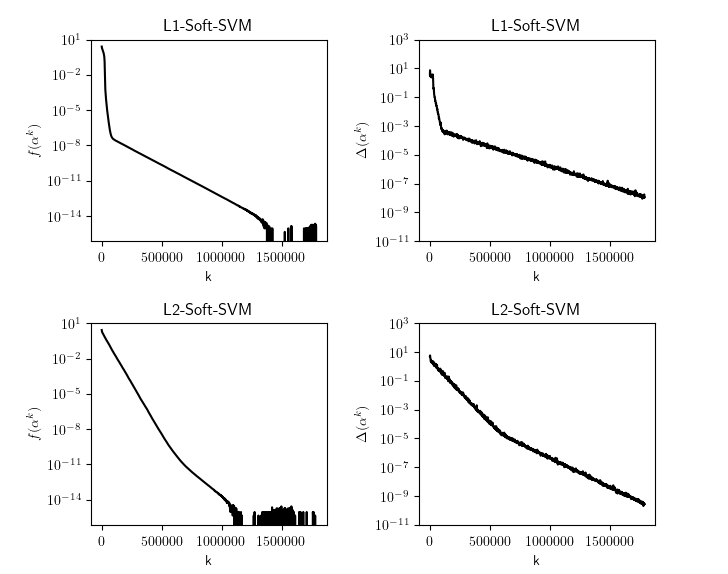
\includegraphics[scale=0.4]{abbildungen/exp-a.png}
	\caption{Konvergenzverhalten der Koordinaten-Abstiesmethode vom $L1-$ und $L2$-Soft-SVM.}
	\label{img:exp-1}
\end{figure}

Zu erkennen ist, dass die Konvergenzrate auf der linken Seite doppelt so hoch ist, wie auf der rechten. Dies geht mit der quadratischen Form der Zielfunktion einher. Weiter deutet das (im Trend) - bis auf den Knick - sehr lineare Verhalten aller Graphen auf eine lineare Konvergenz der Zielfunktion $f$ , sowie $\Delta(\alpha^k)$ hin. Die am Ende auftretenden Fluktuationen der beiden Graphen auf der linken Seite lassen sich mit der maximalen Maschinengenauigkeit von ungefähr $1.1 \cdot 10^-{16}$ erklären.

\section{Experiment B: Einfluss der randomisierten Permutation des Koordinatenabstiegs}
\begin{figure}[htbp]
	\centering
	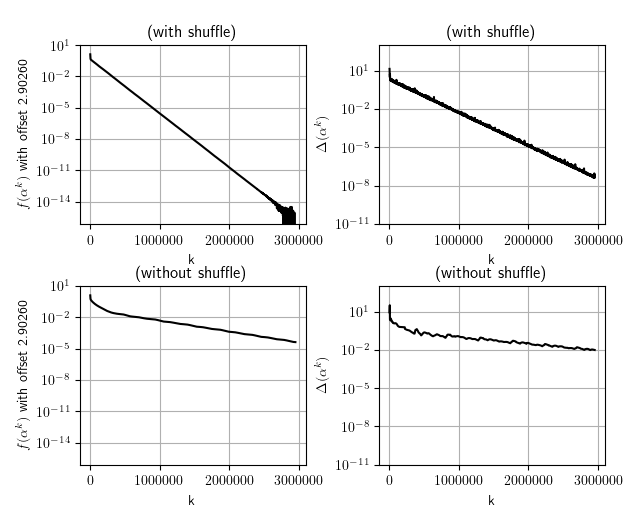
\includegraphics[scale=0.5]{abbildungen/exp-b.png}
	\caption{Konvergenzverhalten der Koordinaten-Abstiesmethode vom $L2$-Soft-SVM einmal mit und einmal ohne der Permutationen-Strategie.}
	\label{img:exp-b}
\end{figure}
Wir wollen nun den Einfluss der zufälligen Permutationen der Koordinaten in einem äußeren Zyklusdurchlauf auf die Konvergenzgeschwindigkeit untersuchen. Hierfür vergleichen wir den L2-Soft-SVM mit und ohne der Permutationen-Strategie. Für dieses Experiment wurden die Kategorien \emph{sci.electronics}, \emph{comp.sys.ibm.pc.hardware} aus dem 20newsgroup-Datenset herangezogen. Für die Parameter des L2-Soft-SVM wurden in beiden Fällen C=1, tol=$10^-9$ und max\_it=2500 gewählt.

Auf der Abbildung \ref{img:exp-b} sind 4 Plots zu erkennen. Die Plots auf der linken Seite wurden mit der Permutationen-Strategie gebildet, die beiden auf der rechten Seite ohne Permutationen-Strategie. Es ist deutlich zu erkennen, dass die Permutationen-Strategie zu einer schnelleren Konvergenz führt.

\section{Experiment C: Textklassifizierung} \label{sec:exp-c}
In diesem Experiment wird die Klassifizierungsgenauigkeitim Sinne der aus Kapitel 1 definierten Metriken, sowie der Trainingszeit für die L1-, L2-Soft-SVM, \emph{LibSVM} \cite{chang-libsvm-11}, und dem multinomialen \emph{Naive-Bayes-Verfahren} verglichen. Die LibSVM löst das duale Problem für die Hard-SVM mit Schlupfvariablen. Für die L1-, L2-Soft-SVM und  LibSVM wurden die Parameter C = 1 und tol = $10^-4$ gesetzt. er resultierende lineare Klassifizierer ordnet jedem Dokument genau eine Klasse zu. Hierfür wurde die one-vs-rest Strategie benutzt. Zu Beginn des Experimentes wurden die Dokumente in ein Trainings- und ein Test-Segment aufgeteilt. In der \emph{Trainingsphase} wurden die Modelle mit den Daten aus dem Trainingssegment erzeugt, für die \emph{Testphase} wurden dann die Trainingsdaten herangezogen. Aus Performance-Gründen wurde für den Test die von scikit-learn bereitgestellte Software \emph{Liblinear} \cite{fan-liblinear-08} und LibSVM benutzt.

\begin{table}[h!]
	\centering
	\begin{tabular}{|l | c | c |}
		\hline
		& neg. klassifiziert & pos. klassifiziert \\
		\hline 
		echt neg. & a & b \\
		\hline 
		echt pos. & c & d \\
		\hline
	\end{tabular}
	\caption{Mögliche Fälle bei einem Binärklassifikator: c stellt den Fehler 1. Art da, b den Fehler 2. Art.}
	\label{tab:fehlerarten}
\end{table}

Als Metriken für die Evaluierung wurden die \emph{Precision} (P), der \emph{Recall} (R) und der F1-Score ($F_1$)  (siehe etwa \cite{f-ir}) für die einzelnen Klassen (one vs. rest) berechnet und anschließend ihr Mittelwert gebildet. Mit der Tabelle \ref{tab:fehlerarten} ergeben sich die Precision aus dem Anteil der korrekt positiv klassifizierten zu allen positiv klassifizierten Testvektoren $(d/(b+d))$, der Recall aus dem Anteil der korrekt positiv klassifizierten zu allen echt positiven Testvektoren ($d/(c+d)$) und der F1-Score zu $F_1 = 0.5 / (P^{-1} + R^{-1})$. \\

Die Resultate zu den einzelnen Klassen wurden in den Tabellen \ref{tab:MNB}, \ref{tab:LibSVM}, \ref{tab:L1SoftSVM} und \ref{tab:L2SoftSVM} zusammengefasst. Tabelle \ref{tab:ml-avg} fasst die gemessenen Mittelwerte (average) der Precision, dem Recall und dem F1-Score, sowie Trainings- und Klassifizierungszeiten (training time/prediction time) zusammen. \\

\begin{table}[h!]
\centering
\begin{tabular}{|l | r | r | r | r| r|}
\hline
                            & precision  & recall & f1-score & train. (s) & pred. (s) \\
\hline
Multinomial Naive Bayes   	&0.76      & 0.76     & 0.74& 0.250 & 0.078 \\
LibSVM   					&0.74      & 0.73     & 0.73& 87.67 & 69.14 \\
L1-Soft-SVM (Liblinear)  &0.78      & 0.78     & 0.78& 12.49 & 0.047 \\
L2-Soft-SVM (Liblinear)  &0.79      & 0.79     & 0.78& 13.09 & 0.042 \\
\hline
\end{tabular}
\caption{Gemessene Genauigkeit, Trainings- und Klassifizierungszeit vom multinomialen Naive-Bayes, LibSVM, $L_1$-Soft-SVM und L2-Soft-SVM für den 20newsgroup-Datensatz. }
\label{tab:ml-avg}
\end{table}

Die Tabelle \ref{tab:ml-avg} zeigt, dass die Textklassifizierung mit der in der Arbeit vorgestellten Implementierung der $L_1$- und L2-Soft-SVM auch im Vergleich zu anderen Verfahren brauchbare Ergebnisse liefert. Außerdem ist erkennbar, dass die Trainingszeiten bei der $L_1$- und der L2-Soft-SVM ähnlich sind. Im Vergleich zur LibSVM sind die Trainingszeiten  deutlich geringer, im Vergleich zum multinomialen Naive-Bayes-Verfahren deutlich höher. Die Klassifizierungszeiten sind beim $L_1$- und L2 am geringsten. Die hohe Klassifizierungszeit bei der LibSVM ergibt sich dadurch, dass bei der Entscheidungsfunktion 
$$
\sign \left( \sum_{i= 1}^{l} y_i \alpha_i K(x_i,x) + b \right)
$$ 
auch im linearen Fall der Kernel $K$ für jede Trainingsinstanz einzeln berechnet wird, siehe hierzu etwa \cite{chang-libsvm-11}.